\documentclass[variant=courcework]{bsuir}
\usepackage{pdfpages}

\graphicspath{{./doc/}}
\hyphenation{mea-sure}
\hyphenation{gaus-sian}

\faculty{компьютерного проектирования}
\departmentlong{инженерной психологии и эргономики}
\departmentshort{эргономики}
\departmentmanager{эргономики}
\worktitle{Создание сервиса поиска визуально схожих изображений в неорганизованных коллекциях}
\workcode{БГУИР КР 1-58 01 01 002 ПЗ}
\titlepageyear{2024}

\begin{document}

\maketitle{Студент\\Руководитель}{Бородин А.Н.\\Кабариха В.А.}

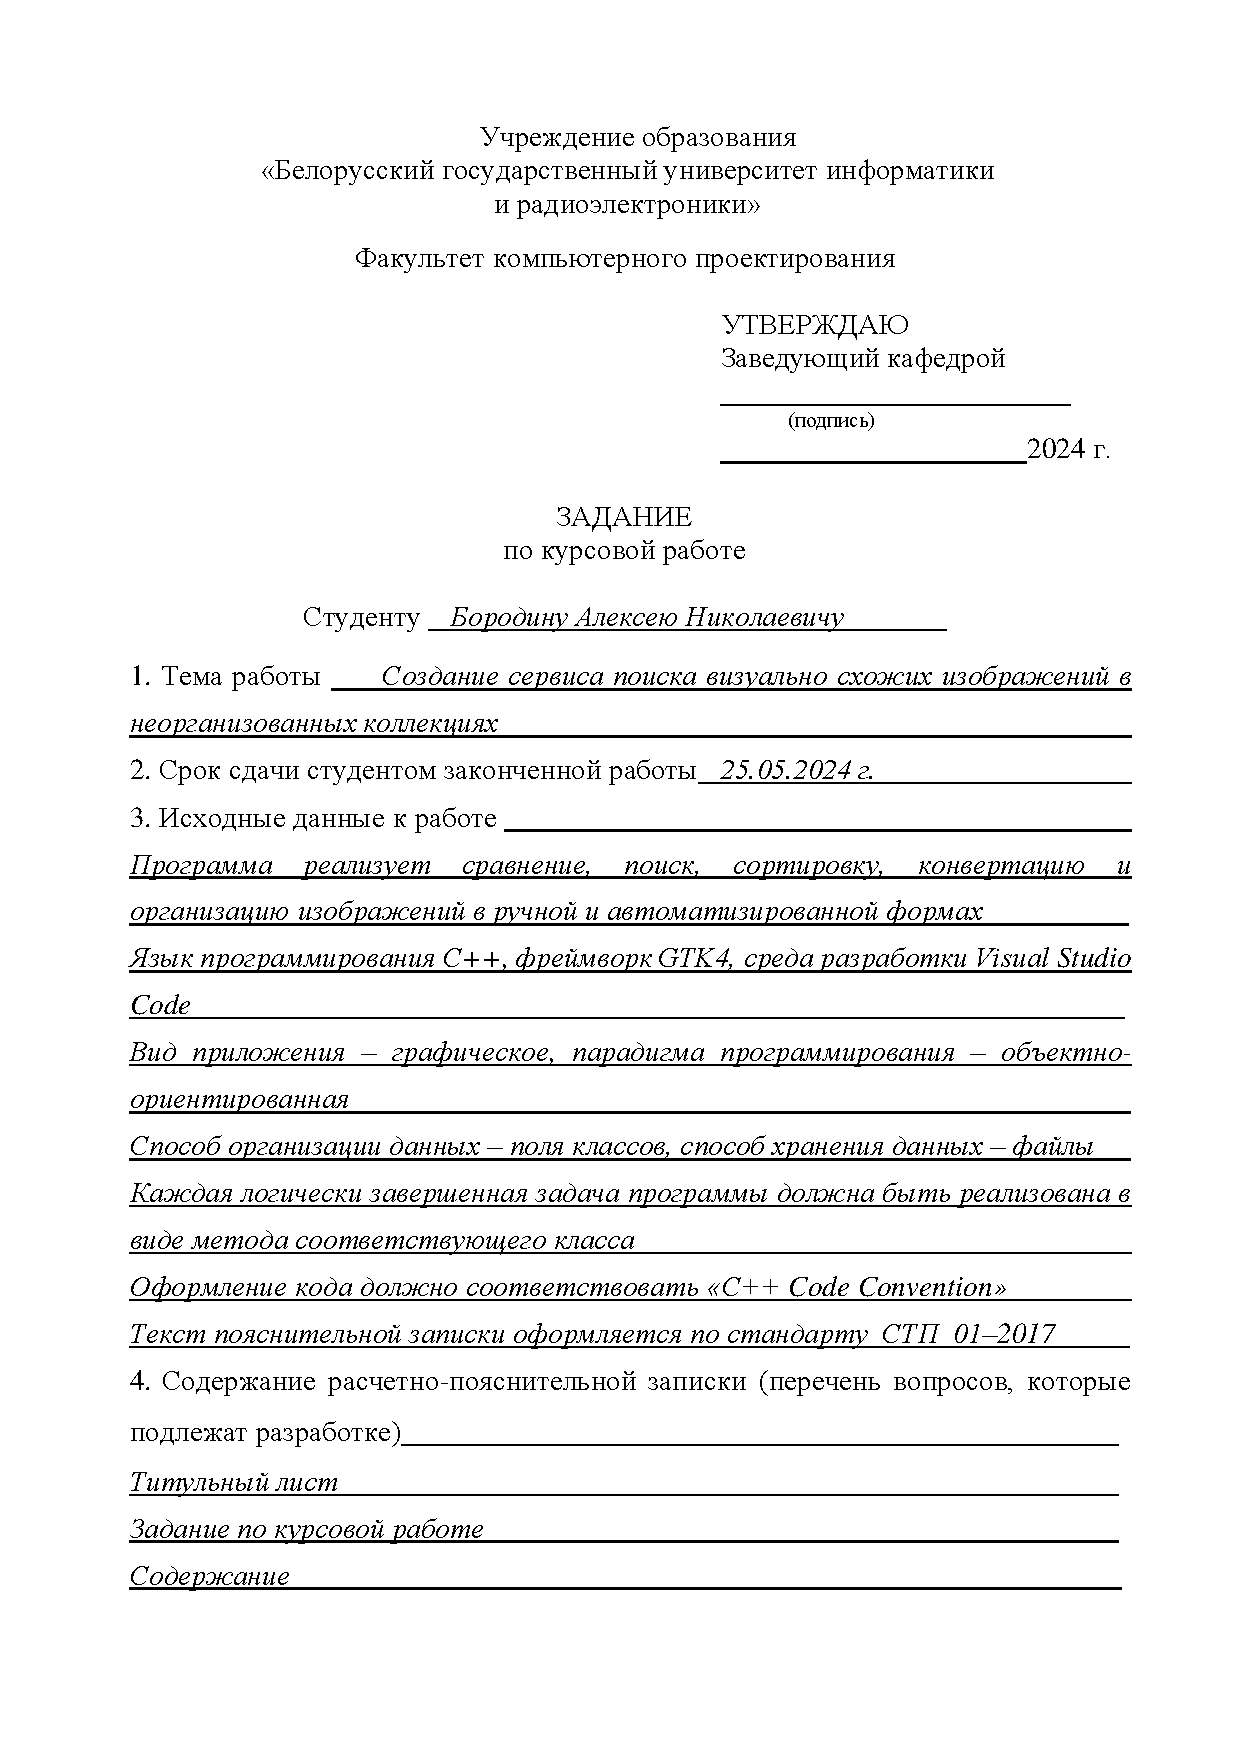
\includepdf[pages=-]{doc/task.pdf}

\tableofcontents

\chapter*{Введение}

Данная курсовая работа выполнена с целью освоения алгоритмов сравнения
изображений, оценки их схожести и вероятности совпадения изображений.
Дополнительной задачей выступает изучение создания программ с графическим
интерфейсом на языке C++ в объекто-ориентированной парадигме. При работе
решались следующие задачи:

\begin{itemize}
    \item изучение алгоритмов сравнения изображений;
    \item изучение фреймворка графического интерфейса;
    \item сравнение изображений;
    \item сравнение группы изображений;
    \item создание выборки файлов по критериям поиска;
    \item группое удаление, переименование и удаление файлов выборки;
    \item поиск дубликатов;
    \item реализация удобного интерфейса.
\end{itemize}

В работе реализован алгоритм нахождения перцептивного хеша (в нескольких
вариантах) и, в его рамках, алгоритм изменения размера изображения. В
\hyperref[sec:2.1]{подразделе 2.1} дана их характеристика.

При подготовке к курсовой работе был проанализирован ряд программ с открытым
исходным кодом, предназначенных для дедубликации: \textquote{rmlint},
\textquote{dupeGuru}, \textquote{Czkawka}.

Разработанная программа может помочь обычным пользователям в процессе
организации их персональной коллекции и разработчикам более крупных программных
продуктов. В роли библиотеки, к примеру, программа может быть использована для
оптимизации базы изображений соцсети, месседжера, файлообменника, поисковика или
же архива.

\chapter{Постановка задачи}

\section{Описание предметной области}

Объем памяти всегда имеет предел, которого, зачастую, не хватает. Для отдельного
пользователя это оборачивается поиском файлов к удалению, а для бизнеса лишними
денежными тратами на расширение своих хранилищ. Для откладывания неизбежного
истощения свободного места непрерывно разрабатываются новые методы сжатия
информации. Дедубликация, удаление дублирующейся информации или замена на ссылку
к другой копии -- один из них.

Одно из самых эффективных решений -- сжатие на уровне файловой системы. Однако,
способные на это современные системы, такие как BTRFS или ZFS, мало
распространены и снижают затраты только в рамках устройства, на котором
установлены. Но, для программ, два файла, прошедшие дедубликацию на этом уровне,
останутся разными файлами, из-за чего объемы используемого сетевого трафика и
количество итераций при обработке выборки файлов останутся теми же.

Одно другого не исключает, но, в большинстве случаев, устранение дубликатов
лучше отдать под ответственность пользовательской программы. Будь то
медиахостинг, социальная сеть, месседжер, датасет или просто личная коллекция.
Если речь идет об сервисе, выполнение программы можно встроить в поток ее
рабочего процесса.

Выборка дубликатов представляет из себя список файлов, так что, поиск дубликатов
можно рассматривать как условие при создание файловой выборки, а удаление -- не
единственная доступная операция для файла. Следовательно, механизм поиска и
удаления дубликатов легко расширяется до системы организации выборок.

Регулярное использование подобной системы наводит порядок в коллекции, упрощает
поиск изображений в ней пользователем и снижает нагрузки на память машины.

% Получение коэффициента разности изображений -- один из фундаментальных вопросов
% области компьютерного зрения, служащий основой для решения задач о создании
% изображения-разности, совмещения нескольких изображений в одно, а за ним и
% генерации изображений, в том числе, и по описанию.

% Сам по себе коэффициент может быть применен, в зависимости от алгоритма, для
% поиска одинаковых изображений, различающихся сжатием или кодировкой, поиска
% дубликатов, перевернутых изображений и для однозначной идентификации
% изображения. В курсовой работе он нужен как параметр создания выборок (выбрать
% дубликаты в каталоге или некого отдельно взятого изображения).

% \subsection{Коэффициент разности изображений и компьютерное зрение}
% \subsection{Среднеквадратическое отклонение}
% \subsection{Мера индекса структурного сходства}
% \subsection{Пиковое соотношение сигнал/шум}

\section{Сравнительный анализ}

\subsection{\textquote{rmlint}}

\makeimage{rmlint.png}[\texttt{rmlint -g}]

Консольная и, с недавних пор, графическая программа для поиска дубликатов общего
предназначения. Для поиска дубликатов используется хеш-функция blake2b.
Дополнительные варианты: paranoid, highway256, metro256, metro (в порядке
возрастания точности). По окончанию работы, программа генерирует скрипт для
удаления найденных файлов. Работает быстро, удобна, не переусложнена лишним
функционалом и имеет много режимов работы и форматов вывода результата. В
сравнении с разрабатывамой программой, не умеет анализировать содержимое
изображений и заниматься их организацией. Написан на C и Python.\\

\url{https://rmlint.readthedocs.io/}

\subsection{\textquote{dupeGuru}}

\makeimage{dupeguru.png}[Интерфейс dupeGuru]

Мощный кроссплатформенный дедубликатор, написанный на Python с использованием
PyQt5. Имеет отдельные алгоритмы для сравнения обычных файлов, музыки и
изображений. Так же, может проводить сравнение по метаданным файлов. Тщательнее
всех конкурентов справляется с задачей, но платит за это низкой скоростью
работы. Никаких функций файловой организации. Имеется кеширование результатов.\\

\url{https://dupeguru.voltaicideas.net/}

\subsection{\textquote{Czkawka}}

\makeimage{czkawka.png}[Интерфейс Czkawka]

Czkawka (переводится с польского как икота) -- наследник заброшенного с 2017
проекта FSlint. В отличии от оригинала, написанного на Python второй версии и
работающего только под линукс-системами, разработан на Rust и поддерживает ОС
Windows и MacOS. В нем реализован не только весь функционал dupeGuru, но и:
поиск пустых файлов и каталогов, больших и временных файлов, похожих видео, не
работающих символьных ссылок, некорректно-записанных файлов и несовпадений
содержимого с расширением файла. Для сравнения изображений используется
перцептивный хеш, параметры вычисления которого можно настроить:

\begin{itemize}
    \item Алгоритм изменения размера изображения: Lanczos3, Nearest, Triangle,
          Gaussian, CatmullRom;
    \item Размер хеша: 8, 16, 32, 64;
    \item Тип хеша: одинарный, вертикальный или двойной градиентный, блочный,
          средний.
\end{itemize}

\url{https://github.com/qarmin/czkawka}

\section{Информационная база задачи}

При выполнении работы источником вдохновения послужили схожие проекты, статьи на
\href{https://habr.com/}{habr.com} из хаба \textquote{Обработка изображений}.

\section{Функциональное назначение}

Требования к программе:

\begin{itemize}
    \item составление списка файлов, удовлетворяющих ряду параметров;
    \item ручное добавление файлов;
    \item изменение текущих параметров поиска;
    \item создание новой выборки в новом окне;
    \item групповое удаление, перенос и переименование файлов;
    \item шаблонирование при задании новых имен и путей файлов и поиске;
    \item открытие изображения в программе просмотра изображений;
    \item указание параметров сравнения изображений;
    \item генерация скриптов для удаления файлов;
    \item графический интерфейс;
    \item консольный интерфейс;
    \item библиотечный интерфейс;
    \item работоспособность под ОС NixOS.
\end{itemize}

\chapter{Проектирование задачи}
\section{Алгоритм решения задачи}
\label{sec:2.1}



\section{Логическое моделирование}



\section{Выбор и обоснование инструментов разработки}



% \chapter{Программная реализация}
% \section{Физическая структура}
% \section{Описание разработанных модулей}
% \chapter{Тестирование}
% \chapter{Применение программы}
% \section{Руководство пользователя}
% \chapter*{Заключение}

\end{document}
